\documentclass{article}

\usepackage{amsthm}
\usepackage{amsmath}
\usepackage{amsfonts}
\usepackage[margin=1in]{geometry}
\usepackage{hyperref}
\usepackage{tikz}
\usepackage{wasysym}

\DeclareMathOperator{\re}{re}
\DeclareMathOperator{\res}{res}


\title{\href{https://math.umn.edu/sites/math.umn.edu/files/exams/complexs19.pdf}{Spring 2019 Complex Analysis Preliminary Exam}}
\author{University of Minnesota}
\date{}
\begin{document}
\maketitle


\begin{enumerate}
	\item Give a conformal mapping from the (open) upper half plane to the slit disk \[ D = \{ z \in \mathbb{C} : |z| < 1, z \not \in [0,1] \}\]
	
	% See PG notes 3.0.3. We are looking for the inverse of the Cayley map.
	% The Cayley transformation according to Wikipedia is the inverse of the Cayley map according to PG
	% See also Mobius transformation which PG calls a fractional linear transform.
	\begin{proof}
		Consider the map $f(z) = \frac{z-i}{z+1}: \mathbb{C} \rightarrow \mathbb{C}$. Note that this is a fractional linear transformation.
		
		Let $H$ be the open upper half plane.
		We first want to show that $f(H) = D$.
		
		First, when we restrict $f$ to the real line, we see $\lim_{x \rightarrow \pm \infty} f(x) = 1$. We also see that 
		\begin{align*}
			f(1) &= \frac{1-i}{1+i}\\
				&= \frac{(1-i)^2}{ | 1+i|^2}\\
				&= \frac{1-2i-1}{ (\sqrt{2})^2}\\
				&= -2i/2 \\
				&= -i
		\end{align*}
		and
		\begin{align*}
			f(-1) &= \frac{-1-i}{-1+i}\\
				&= \frac{(-1-i)^2}{|-1+i|^2}\\
				&= \frac{1 + 2i - 1}{ (\sqrt{2})^2 }\\
				&= +i
		\end{align*}
		finally
		\[f(+i) = \frac{i - i }{i+i} = 0.\]
		Thus, because fractional linear transformations preserve circles-and-lines, and $+i \in H$ gets mapped to the interior of $D$, then $f(H) = D$.

		Now we show that $f(z)$ is conformal on the open upper half plane. $f$ is conformal where its derivative is nonzero, and so we compute
		$f^\prime = \frac{(z+1)- (z-i)}{(z+1)^2} = \frac{1-i}{(z+1)^2}$, which is defined except at $z=-1$ (which is not in the open upper half plane so we need not worry) and is nonzero wherever it is defined.
		Thus, $f$ is a conformal mapping from $H$ to $D$.
		 
	\end{proof}
	
	\newpage
	
	\item Write the first three terms of the Laurent expansion of $\displaystyle f(z) = \frac{1}{z^5-1}$ centered at $0$ and convergent in $|z|<1$.
	
	\begin{proof}
		Observe that \[\frac{1}{z^5-1} = \frac{-1}{1-z^5} = -\sum_{n=0}^\infty z^{5n}\]
		which converges for $|z^5|<1$ which is $|z|^5<1$ or $|z|<1$. 
		Thus, the first three nonzero terms of the expansion of $f$ are 
		$a_0 = -1$, $a_5=-1$, and $a_{10} = -1$.
	\end{proof}
	
	\item Classify entire functions $f$ such that $|f(z)| \leq 1 + \sqrt{|z|}$
	
	\item Evaluate $\displaystyle \int_{-\infty}^\infty \frac{\sin(x)}{1+x^2} dx$
	
	\begin{proof}
		Let $f: \mathbb{C} \rightarrow \mathbb{C}$ be given by $f(z) = \frac{-i e^{iz}}{1+z^2}.$ 
		When we restrict to $x \in \mathbb{R}$, we have 
		$f(x) = \frac{-ie^{ix}}{1+z^2} = \frac{-i(\cos x + i \sin x)}{(z+i)(z-i)}$ and so $f$ has real part $\re f(x) = \frac{\sin(x)}{1+x^2}$.
		Thus, the real part of the integral $\re \left (\int_{-\infty}^{\infty} f(z) dz \right)$ is the integral we wish to compute.
		
		Note that the numerator of $f$ is entire and the denominator is also entire and is only $0$ at $z = \pm i$.
		
		Let $t>0$ and let $\gamma_t$ be the curve given by the union of $[-t,t] \subset \mathbb{R}\subset \mathbb{C}$ with the upper half-circle of radius $t$, with positive orientation. 
		Visually:
		\begin{center}
		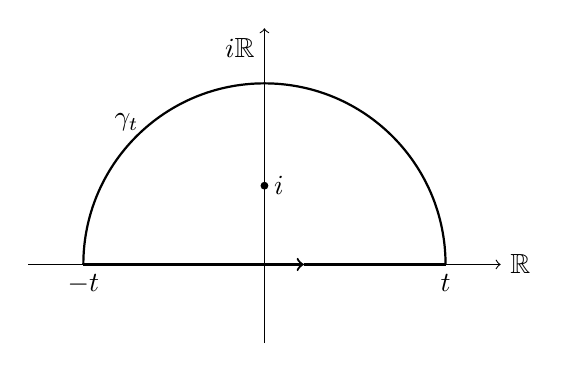
\begin{tikzpicture}
			%\draw[step=1cm,gray,very thin] (-2.9,-0.9) grid (2.9,2.9);
			\draw[thin,->] (0,-1) -- (0,3); 
			\draw[thin,->] (-3,0) -- (3,0);
			
			\node[anchor = north east] at (0,3) {$i \mathbb{R}$};
			\node[anchor = west] at (3,0) {$ \mathbb{R}$};
			
			\node[fill = black, inner sep=1pt, circle] at (0,1) {};
			\node[anchor = west] at (0,1) {$i$};
			
			\node[anchor = north] at (2.3,0) {$t$};
			\node[anchor = north] at (-2.3,0) {$-t$};
			
			\node at (-1.75,1.8) {$\gamma_t$};
			
			\draw[thick] (2.3,0) arc (0:180:2.3) ;
			\draw[thick,->] (-2.3,0) -- (0.5,0) ; 
			\draw[thick] (0.5,0)--(2.3,0);
		\end{tikzpicture}
		\end{center}
		
		Since $f$ is holomorphic on and inside $\gamma_t$ except at $i$, which is a simple pole
		the residue theorem tells us that 
		$\int_{\gamma_t} f(z) dz = 2\pi i \res_{i} f(z)$.
		
		To compute $\res_i f(z)$, take $\lim_{z \rightarrow i} (z-i) f(z) = \lim_{z \rightarrow i} \frac{-ie^{iz}}{z+i} = \frac{-i}{e (2i)} =\frac{-1}{2e}$
		
		So then $\int_{\gamma_t} f(z)dz = -\frac{\pi i}{e}$.
		
		We can split the integral into the part along $[-t,t]$ and along $C_t$, the upper half-circle of radius $t$, as
		\[ \int_{\gamma_t} f(z) dz = \int_{[-t,t]} f(z) dz + \int_{C_t} f(z) dz.\]
		We can use the estimation lemma to bound the magnitude of integral over the half-circle as 
		\begin{align*}
			|\int_{C_t} f(z) dz |&\leq \pi t \sup_{z \in C_t} |f(z)|.
		\end{align*}
		To compute 
		\begin{align*}
			\sup_{z \in C_t} |f(z)| &= \sup_{z \in C_t} \left | \frac{-ie^{iz} }{1+z^2} \right |\\
			&= \sup_{z \in C_t} \frac{|e^{iz} |}{|1+z^2|} \\
		\end{align*}
		When we consider $z = x+iy \in C_t$, we see that $|e^{iz}| = |e^{i(x+iy)}| = | e^{ix-y} | = e^{-y} \leq 1$
		so 
		\begin{align*}
			\sup_{z \in C_t} \frac{|e^{iz} |}{|1+z^2|} & \leq \sup_{z \in C_t} \frac{1}{|1+z^2|} \\
			&\leq \sup_{z \in C_t} \frac{1}{||z^2|- |-1||} & (\text{reverse triangle inequality})\\
			&= \sup_{z \in C_t} \frac{1}{| |z^2| - 1|}\\
			&= \sup_{z \in C_t} \frac{1}{| t^2 -1 |}\\
			&= \frac{1}{|t^2-1|}.
		\end{align*}
		
		Thus, we have
		\[ \left |\int_{C_t} f(z) dz \right |\leq \pi t \frac{1}{|t^2-1|}  \]
		and taking the limit $t \rightarrow \infty$ we see
		\[ \lim_{t \rightarrow \infty} \int_{C_t} f(z) dz = 0.\]
		Thus, in the limit
		\[ \lim_{t \rightarrow \infty} \int_{\gamma_t} f(z) dz = \lim_{t \rightarrow \infty} \int_{[-t,t]} f(z) dz = \int_\mathbb{R} f(z) dz.\]
		The integral over $\gamma_t$ was independent of $t$ (thanks residue theorem \smiley{}), so we see
		\[ \int_\mathbb{R} f(z) dz = \frac{-\pi i}{e}.\]
		We wanted to compute the real part
		\[ \int_\mathbb{R} \frac{\sin x}{1+x^2} dx = 0.\]
		
		We could also see that $1+x^2$ is an even function and $\sin(x)$ is an odd function so $\sin(x)/(1+x^2)$ is an odd function, 
		so its integral must be 0, but why do that when we could use the residue theorem \smiley{}.
	\end{proof}	
	
	\setcounter{enumi}{4}
	
	\item Determine the radius of convergence for the power series of $\sqrt{z}$ at $z_0 = -3 + 4i$.
	
	\begin{proof}
	The radius of convergence of the power series of $\sqrt{z}$ is the radius of the largest disk for which there is a holomorphic function which agrees with $\sqrt{z}$.
	%
	Recall that we define complex exponentiation by $z^\alpha := e^{\alpha \log z}$, so $\sqrt{z} = e^{\log(z)/2}$. Composition of holomorphic functions is holomorphic, so since $e^w$ is entire, the radius of convergence is limited by $\log(z)$. 
	
	There is no number $w \in \mathbb{C}$ such that $e^w = 0$, and so there is no possible way to have a holomorphic logarithm at $0$. This bounds the radius of convergence by $|-3 + 4i - 0|=5$. 
	
	On the other hand, it is a theorem\footnote{Theorem 6.1 in Chapter 3 of Stein and Shakarchi's \textit{Complex Analysis}} that if $\Omega$ is simply connected and does not contain $0$, then there is a branch of the logarithm which is holomorphic on $\Omega$. Consider the open disk $D$ of radius $5$ and centered at $-3 + 4i$. Clearly $D$ does not contain $0$, and so there is a logarithm (call it $\log_D$) which is holomorphic on $D$. Thus, we have a disk of radius $5$ on which there is a holomorphic function $\log_D$ which agrees with $\log$, and so the radius of convergence is \textit{at least} 5. 
	
	Since we know the radius of convergence is both at least 5 and less than or equal to 5, we see that the radius of convergence of the power series for $\log$ is in fact $5$.
	
	\end{proof}
	
	\setcounter{enumi}{7}
	
	\item Define $f(z)$ near $0$ by $f(z)^2 = \frac{\sin z}{z}$. What is the radius of convergence of the power series of $f$ at $0$.
	
%	\begin{proof}
%		Since $f(z)^2 = \frac{\sin z}{z}$, then $f(z) = \frac{(\sin z)^{1/2}}{z^{1/2}}$. 
%		Recall that we define exponentiation in $\mathbb{C}$ to be $z^\alpha = e^{\alpha \log z}$, and so we have that 
%		\[ f(z) = \frac{e^{\log(\sin(z))/2}}{e^{\log(z)/2}} \]
%		
%		$\log(0)$ is never defined so we need to look where $\sin(z)=0$, which is at $z = \pi n$ for $n \in \mathbb{Z}$. Thus, if we call the radius of convergence $R$, we see that $R \leq \pi$.
%	\end{proof}
%	
%	\begin{proof}
%		Since $f(z)^2 = \frac{\sin z}{z}$ then we have $f(z) = \sqrt{\frac{\sin z}{z}}$ which we interpret as
%		\[ f(z) = e^{ \log (\sin z/z)/2 } \]
%		Thus, the obstruction to analyticity occurs dependent on the term $\log(\sin z/z)$.
%		First, note that $\sin z/z$ has a removable singularity at $z=0$ since
%		$\lim_{z \rightarrow 0}\frac{\sin z}{z} = \lim_{z \rightarrow 0} \frac{\cos z}{1} = 1$. Thus, $\log(\sin z/z)$ can be holomorphically extended in a simply connected disk centered at $z=0$ provided $\sin z/z$ is nonzero. Thus, an upper bound for the radius of convergence is $\pi$ since $\sin (\pi)/\pi = 0$.
%	\end{proof}
%	
%	\begin{proof}
%		Suppose that there were a holomorphic function satisfying $f(z)^2 = \sin z /z $ look at power series expansions
%		Then %\[f(z) = \sum_{n \
%	\end{proof}
%		
%	Hmm. Interesting. Is this well defined? I think so because complex.
%	Maybe its all of C? Theres definitely a pole at $0$, but $z^{1/2}$ is entire, $\sin z$ is entire, so $\sqrt{\sin z}$ is entire.
%	
%	The power series expansion of $1/z$ converges except at $0$, and so $1/\sqrt{z}$ is analytic except at $0$. Then the product is analytic so $\sqrt{\frac{\sin z}{z}}$ is analytic. 
%	
%	There is a theorem that if $f$ is nonvanishing on $\Omega$ then there is a g so that $f = e^g$.
%	
%	Does the branch cut force the radius of convergence (since centered at $0$) to be $R=0$?
%	
%	There is a removable discontinuity at $z=0$, which can be fixed by $f(0) = \pm 1$. Is this function well defined? if not well defined then certainly can't be convergent.
\end{enumerate}


\end{document}